\begin{landscape}
	\section{Grobkonzept}
		\begin{figure}[h!]
			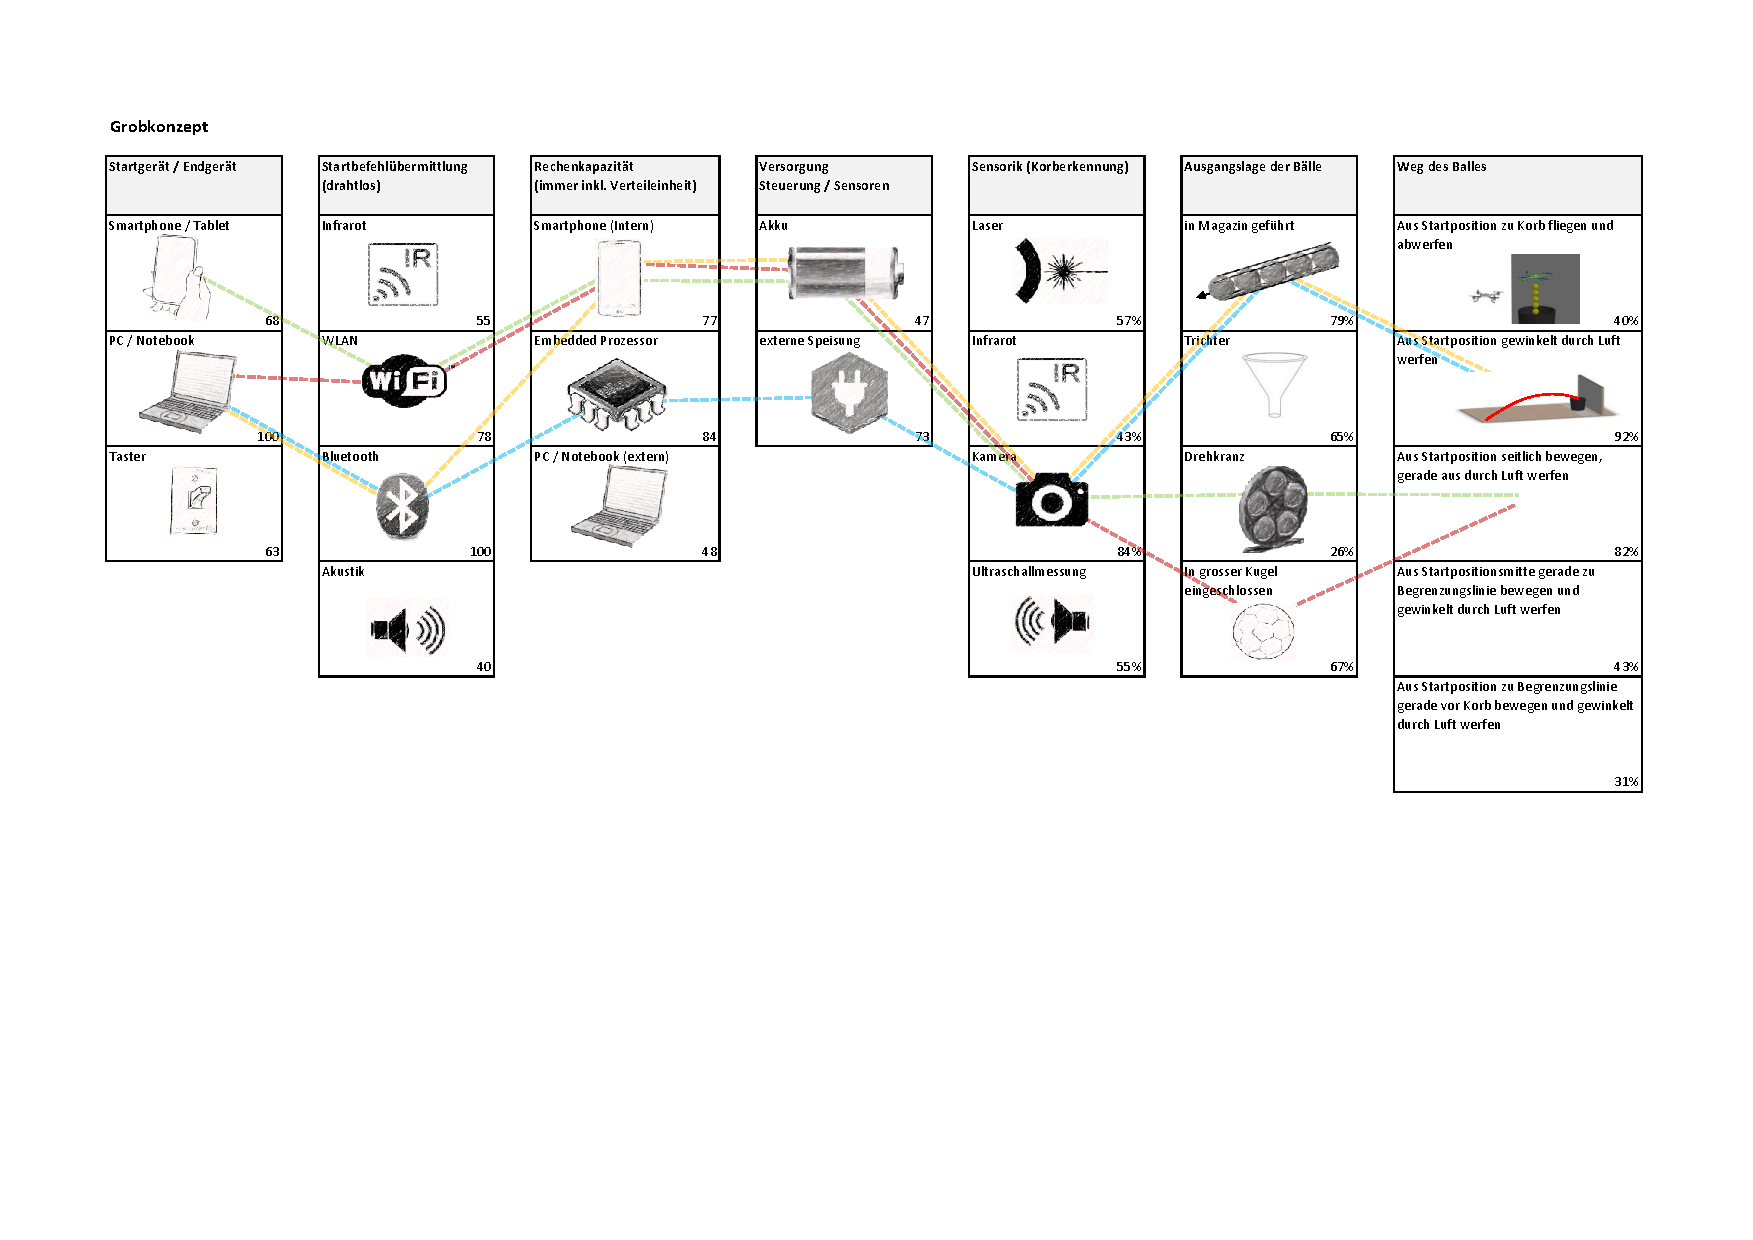
\includegraphics[page=1,scale=0.75,clip,trim=17mm 37mm 21mm 19mm]{Morphologie/Bilder/Grobkonzept.pdf}
			\centering
			\caption{Grobkonzept} 
			\label{abb:Grobkonzept}
		\end{figure}	
\end{landscape} 

\parindent0pt{\textit{Die detaillierte Bewertung aller Varianten sind dem Anhang \ref{apx:BewertungGrobkonzepte} zu entnehmen.}}\\
\\
Es wurden vier Varianten (orange, grün, rot, blau), wie in Abbildung \ref{abb:Grobkonzept} ersichtlich, gewählt. 
\begin{itemize}
	\item Blaue Variante\\
	Eine Auswahl aller Lösungen, welche die höchste Punktezahl durch die Bewertungskriterien erreichte.
	
	\item Rote Variante\\
	Ausgangspunkt in dieser Variante ist die Auswahl, die Bälle in eine Kugel einzuschliessen. Da ein Smartphone mit integrierter Kamera verwendet wird, kann man zwei Teilprobleme mit einem Gerät lösen. Den Weg des Balles via seitliche Verschiebung wurde aufgrund der Unhandlichkeit der grossen Kugel gewählt: der Weg soll kurz und einfach gehalten werden. Der Akku dient in dieser Variante neben der Energieversorgung auch als Ballast, um dem grossen Gewicht der Kugel entgegenzuwirken. Weiter ist die Ausgabe des Startsignals mit einem Notebook, sowie die Übertragung mit WLAN leicht zu Realisieren, da diese Lösungen auf gut dokumentierten Technologien basieren.
	
	\item Grüne Variante\\
	Für die grüne Variante wurde als Ausgangslage der Bälle die Führung in einem Drehkranz gewählt. Kongruent zur Variante Rot, wurde auch hier der Weg des Balles via seitliche Verschiebung aufgrund der Unhandlichkeit des Drehkranzes als Favorit erkoren. Für die Wahl des Akkus, der Startsignal-Übertragung per WLAN und die Verwendung eines Smartphones überzeugten dieselben Kriterien, welche bereits in der roten Variante genannt wurden.
	
	\item Orange Variante\\
	Aus der Startposition gewinkelt werfen, ist der Ursprung der orangen Variante. Eine geführte Ausgabe aus einem Magazin hat den Vorteil, dass es mit leichten Materialen gebaut werden kann, verschiedene Formen, Winkel und Ausgabegeschwindigkeiten zur Verfügung stehen. Der Akku dient in dieser Variante neben der Energieversorgung auch als Ballast und hat den schönen Nebeneffekt, dass das System energieautark ist.
\end{itemize}

\subsection{Entscheidung}
Die orange Variante bietet als gesamtes Konzept die erfolgversprechendste und effizienteste Lösung, bezüglich der vordefinierten Ziele der Team-Charta. Den Ball von der Startposition aus gewinkelt durch die Luft zu werfen erfordert keine zusätzlichen Bauteile um das Produkt am Boden zu verschieben. Dies minimiert einerseits den Aufwand und verringert die Fehleranfälligkeit erheblich. Die Bälle in der Ausgangslage in einem Magazin zu führen hat den Vorteil, dass eine allfällige stückweise Ausgabe der Bälle mit wenig Aufwand hinzugefügt werden kann. Ein Smartphone mit integrierter Kamera löst die zwei Teilprobleme der Korberkennung und Rechenkapazität mit einem Gerät. Des weiteren wäre das Produkt durch die Verwedung eines Akkus energieautark. Die Ausgabe des Startsignals und Endsignals mit einem Notebook und die Übermittlung mit Bluetooth sind einfach auszuführen und beruhen auf wohlbekannten, gut dokumentierten Technologien.